% last updated in April 2002 by Antje Endemann
% Based on CVPR 07 and LNCS, with modifications by DAF, AZ and elle, 2008 and AA, 2010, and CC, 2011; TT, 2014; AAS, 2016

\documentclass[runningheads]{llncs}
\usepackage{graphicx}
\usepackage{amsmath,amssymb} % define this before the line numbering.
\usepackage{ruler}
\usepackage{color}
\usepackage{caption}
\usepackage{subcaption}
\usepackage{bm}
\usepackage{float}
\captionsetup{compatibility=false}
\usepackage[width=122mm,left=12mm,paperwidth=146mm,height=193mm,top=12mm,paperheight=217mm]{geometry}
\begin{document}
% \renewcommand\thelinenumber{\color[rgb]{0.2,0.5,0.8}\normalfont\sffamily\scriptsize\arabic{linenumber}\color[rgb]{0,0,0}}
% \renewcommand\makeLineNumber {\hss\thelinenumber\ \hspace{6mm} \rlap{\hskip\textwidth\ \hspace{6.5mm}\thelinenumber}}
% \linenumbers
\pagestyle{headings}
\mainmatter
\def\ECCV18SubNumber{***}  % Insert your submission number here

\title{Photo-realistic Style Transfer for Videos} % Replace with your title

\titlerunning{ECCV-18 submission ID \ECCV18SubNumber}

\authorrunning{ECCV-18 submission ID \ECCV18SubNumber}

\author{Michael Honke, Rahul N. Iyer and Dishant Mittal}
\institute{University of Waterloo, ON, Canada}


\maketitle

\begin{abstract}
In this paper we present an algorithm to do photo-realistic style transfer on a video given a reference image. Photo-realistic style transfer is a technique which transfers colour from one reference domain to another domain by using deep learning and optimization techniques. Here, we present a technique which we use to transfer style and  colour from a reference image to a video. Optical flow is used to maintain consistent style transfer over multiple frames of video.
\keywords{style transfer, video, optimization, image segmentation, photo-realistic style transfer, videos, optical flow}
\end{abstract}


\section{Introduction}


%This document serves as an example submission. It illustrates the format
%we expect authors to follow when submitting a paper to ECCV. 
%At the same time, it gives details on various aspects of paper submission,
%including preservation of anonymity and how to deal with dual submissions,
%so we advise authors to read this document carefully.

Parameters such as time of day and season often have significant impact on the meaning of images. They don't change the content of an image, but are part of the image's style. Adjusting these details after an image is captured is non-trivial. Furthermore, adjusting such parameters for a video sequence adds additional complexity to the problem. We show how to transfer the style from one photorealistic image to a whole video sequence using deep learning based style transfer. We make use of two prominent works in style transfer.

Ruder et al. \cite{10.1007/978-3-319-45886-1_3} presented a technique which enables the transfer of style from an artistic image (for instance, a painting) to a complete video sequence. They extended static style transfer developed by  Gatys et al. \cite{gatys2016image} and  Johnson et al.\cite{johnson2016perceptual} to complete video sequences. They demonstrated that a naive implementation, independently processing each frame of the video, leads to glimmering and untrue irregularities. This was because the solution of the style transfer task was not steady. With the goal of stabilizing the transfer process and preserving an even transition between independent video frames, they established a temporal constraint that penalized divergence between two consecutive frames. This temporal constraint used the optical flow present in the original video and applied a penalty to the divergence between frames along pixel trajectories. Non-concealed regions and the boundaries of the motion were eliminated from the penalizer. This imparted the liberty to rerender the unconcealed regions and deformed motion boundaries while conserving the look of the rest of the image.

Luan et al. \cite{luan2017deep} developed a deep-learning technique particularly for style transfer in photorealistic images. They reliably transplanted style from a reference image to a content image while preventing the content from being distorted. Their primary contribution was to restrict the style transfer to be locally affine in colorspace, and to depict this restriction as a custom and completely differentiable loss function. They proved that their technique successfully prevents distortions and produces convincing photorealistic style transfers over a wide variety of content, including transfer of parameters like time of day, season, weather and artistic edits. They utilised the Matting Laplacian to restrict the conversion from the input to the output to be locally affine in colorspace. Furthermore, they used semantic segmentation to enable style transfer between like content only.

In our implementation we merge the loss functions and optical flow method used by Luan et al.\cite{luan2017deep} and Ruder et al. \cite{10.1007/978-3-319-45886-1_3} to get a cumulative loss function. This is used to transfer style from a photorealistic reference image to an entire video sequence.

\section{Algorithm}
Ruder et al.'s \cite{10.1007/978-3-319-45886-1_3} main aim is to render a video of stylized images $x$ describing the style of an image $a$ and the content of  video frames $p$. Gatys et al. \cite{gatys2016image} derived an energy minimization problem consisting of a content loss and a style loss. The central concept is that attributes extracted by a convolutional neural network (CNN) contain details about the content of the image, whereas the correlations of these attributes store the details related to style. The expected loss can be minimized by iteratively updating an initially randomized noise image. If each frame is independently processed than this iterative optimization process doesn't consistently style the same objects across frames. To solve this problem Ruder et al. \cite{10.1007/978-3-319-45886-1_3}  created a temporal consistency loss using optical flow. A forward-backward consistency check of optical flow is performed so that style transfer can be initialized for recently disoccluded objects. After which further deviations in these objects' appearances will be penalized. A similar process is done for motion boundaries. The temporal loss given is 
\begin{equation}
	\mathcal{L}_{temporal} (\bm{x}, \bm{\omega}, \bm{c}) = \frac{1}{D} \sum_{k=1}^{D} c_k \cdot (x_k - \omega_k)^2
\end{equation} 
where $\bm{c} \in [0, 1]^D$ is the weight per pixel, zero for recently disoccluded pixels, or those at motion boundaries, otherwise it is one. $D$ is the total number of pixels (across all colour channels). $\bm{\omega}$ is the optical flow of a previous frame warped to the current one $\bm{x}$.

On each iteration the image is processed by the CNN to update the loss functions. Ruder et al.'s complete loss function is then
\begin{equation}
\begin{split}
\mathcal{L}_{video}(f^{(i)} ,a,x^{(i)}) = \alpha \mathcal{L}_{content}(f^{(i)},x^{(i)})
+ \beta \mathcal{L}_{style}(a,x^{(i)})\\+  \gamma \sum_{j \epsilon J, (i-j) \geq 1} \mathcal{L}_{temporal}(x^{(i)}, w_{i-j}^{i}(x^{i-j}),c^{(i-j, i)})
\end{split}
\end{equation}
where i denotes the index of a frame, f\textsuperscript{(i)} is the i\textsuperscript{th} frame of the video, a is the style image, x\textsuperscript{(i)} is the i\textsuperscript{th} stylized frame to be generated, c denotes temporal weight, $\omega$ is a function that warps a given frame using the optical flow field that was estimated between two images. J denotes the set of indices each frame should take into account relative to the frame number, e.g., with J = {1, 2, 4}, frame i takes frames i$-$1, i$-$2, and i$-$4
into account. Taking the temporal loss over multiple previous frames allows for a long term temporal loss to be established. $\mathcal{L}$\textsubscript{content} and $\mathcal{L}$\textsubscript{style} are defined by Gatys et al. \cite{gatys2016image}

Luan et al. \cite{luan2017deep}, apart from $\mathcal{L}$\textsubscript{content} and $\mathcal{L}$\textsubscript{style} described above, explain how to regularize these losses to preserve the structure of the input image and generate outputs that are photorealistic. Rather than directly imposing this constraint on the output image they applied it on the transformation which has been applied to the input image. Describing the space of photorealistic images is a problem that remains unsolved. However, the authors proposed that we don't actually need to solve it if we leverage the fact that the input that would be fed into the model is already photorealistic. Their plan was to assure that this fact should not get lost during the transfer process by attaching a term to the equation of the original loss function which penalizes image deformations. The proposed solution was to search for the transform of an image that is locally affine in color space. That means to search for a function such that for every output there exists an affine function that maps the corresponding RGB components in input to their output equivalents. They build upon the Matting Laplacian of Levin et al. \cite{levin2006closed}. They proposed the following loss function
\[\mathcal{L}_m = \sum_{c = 1}^3 V_c [O]^T M_I V_c [O] \]

where M\textsubscript{I} is a standard linear system that only depends on the input image I and V\textsubscript{c}[O] is the vectorized version (N × 1) of the output image O. M\textsubscript{I} is calculated by first finding the Matting Laplacian of the content image.

One limitation of the style loss presented by Gatys et al. \cite{gatys2016image} was that  the Gram matrix is computed over the entire image. A precise distribution of feature maps is completely encoded by the Gram matrix up-to an isometry. However, this can cause “spillovers” as that limits its power to adapt to variations in semantic context. The solution to this problem was that by keeping the set of labels constant (i.e. sky, buildings, water, etc.) Luan et al. \cite{luan2017deep} generated image segmentation masks for both the input as well as reference images. They included the masks to the input image as supplementary channels and by appending the segmentation channels they built up the neural style algorithm. Finally that style loss was updated as follows

\[ \mathcal{L}_{s+}^l = \sum_{c = 1}^C \frac{1}{2N_{l,c}^2} \sum_{i,j} (G_{l,c}[O]-G_{l,c}[S])_{i,j}^2 \]

where $C$ is the number of channels in the semantic segmentation mask, $S$ is the style image and $G$ is the Gram matrix. Finally they formulated the photorealistic style transfer loss function by combining all 3 components losses together as

\[ \mathcal{L}_{total} = \sum_{1=1}^L\alpha_l \mathcal{L}_c^l + \tau \sum_{1=1}^L\beta_l \mathcal{L}_{s+}^l + \lambda \mathcal{L}_m \]

where L is the total number of convolutional layers and l indicates the l\textsubscript{th} convolutional layer of the deep neural
network, $\tau$ is a weight that controls the style loss. $\alpha$ and
$\beta$ are the weights to configure layer preferences. $\lambda$ is a
weight that controls the photorealism regularization.

To implement the style transfer from one photorealistic image to a whole video sequence using deep learning we merged the concepts from both the works i.e from Ruder et al. \cite{10.1007/978-3-319-45886-1_3} and Luan et al. \cite{luan2017deep}. Precisely, we accomplished this in two parts: 

\begin{itemize}
\item We integrated the loss functions used in photorealistic style transfer  to the loss functions used in artistic video style transfer. After reviewing their implementations, our program was written using the framework of the video transfer algorithm. The style loss of the video method was replaced with that of the photorealistic one. New to the video transfer algorithm was the photorealistic affine transform constraint.

\item  We used a neural network to perform semantic segemnetation on the reference image and all the frames of the video. This helped us to automate the task of segmentation which can then be used in computing the overall loss for the videos. The style loss term in artistic style transfer in videos is replaced completely with the semantic segmentation loss used by Luan et al. \cite{luan2017deep}. The final loss function can be written as
\begin{equation}
\begin{split}
 \mathcal{L}_{final} = \sum_{1=1}^L\alpha_l \mathcal{L}_c^l + \tau \sum_{1=1}^L\beta_l \mathcal{L}_{s+}^l + \lambda \mathcal{L}_m \\ + \gamma \sum_{j \epsilon J, (i-j) \geq 1} \mathcal{L}_{temporal}(x^{(i)}, w_{i-j}^{i}(x^{i-j}),c_{long}^{(i-j, i)})
\end{split}
\end{equation}
 where the symbols are as defined in the previous sections.

Deepflow \cite{weinzaepfel2013deepflow} was used to compute the optical flow of the different frames in the video. To get the segmentation of a particular image we trained a neural network on the ADE20K dataset \cite{zhou2017scene} which provides 20,210 annotated images for training, 2000 for validation and 3000 images for testing for 900 different types of categories defined in SUN database \cite{xiao2010sun}. We trained a Dilated ResNet-34 architecture. By training this we get an IOU of 74.9\% on the validation set. As our style transfer algorithm is dependent on the segmentation, if the model has problem segmenting the image the algorithm also struggles.
\end{itemize}

\section{Results}

The presented method is used to convert a daytime time-lapse of the Eiffel tower to a sunset equivalent using a sunset reference image of the tower.
\begin{figure}[h!]
\centering
\begin{subfigure}[t]{0.3\linewidth}
    \centering
    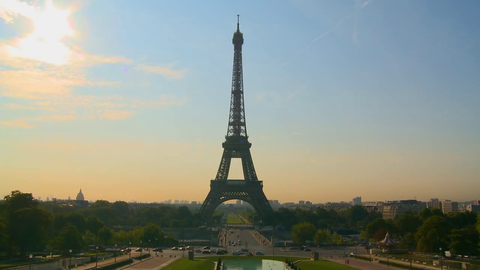
\includegraphics[width=1\linewidth]{small_0014.png}
    \caption{Content Frame 14}
\end{subfigure}
\begin{subfigure}[t]{0.3\linewidth}
    \centering
    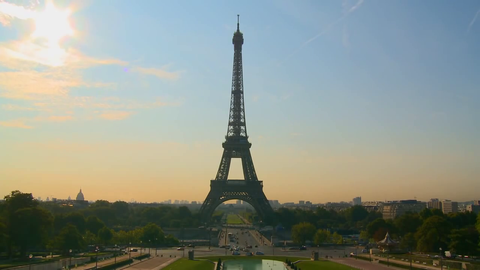
\includegraphics[width=1\linewidth]{small_0031.png}
    \caption{Content Frame 31}
\end{subfigure}
\begin{subfigure}[t]{0.3\linewidth}
    \centering
    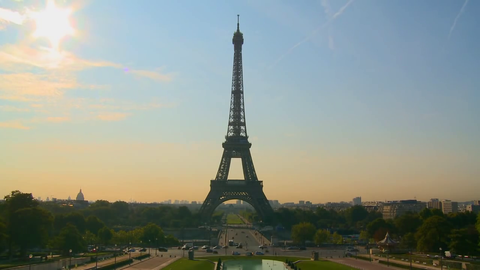
\includegraphics[width=1\linewidth]{small_0052.png}
    \caption{Content Frame 52}
\end{subfigure}

\begin{subfigure}[t]{0.3\linewidth}
    \centering
    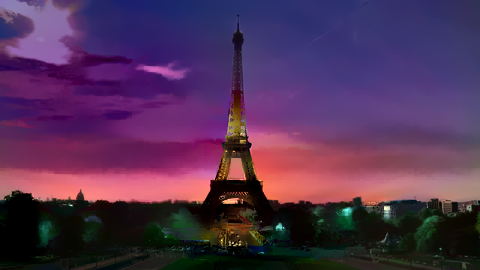
\includegraphics[width=1\linewidth]{best14.png}
    \caption{Output Frame 14}
\end{subfigure}
\begin{subfigure}[t]{0.3\linewidth}
    \centering
    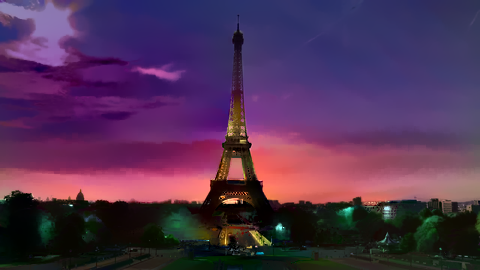
\includegraphics[width=1\linewidth]{best31.png}
    \caption{Output Frame 31}
\end{subfigure}
\begin{subfigure}[t]{0.3\linewidth}
    \centering
    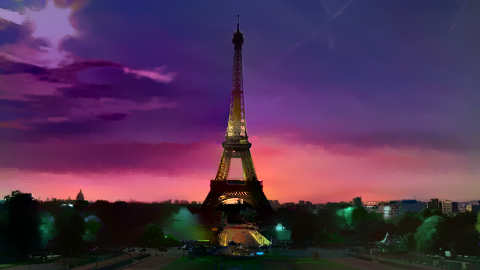
\includegraphics[width=1\linewidth]{best52.png}
    \caption{Output Frame 52}
\end{subfigure}
\begin{subfigure}[t]{0.3\linewidth}
    \centering
    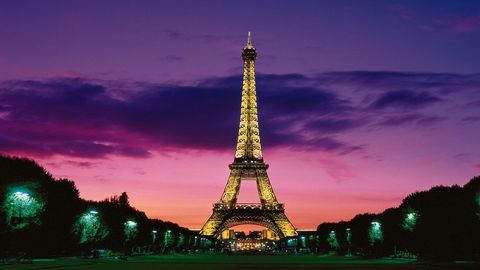
\includegraphics[width=1\linewidth]{reference_paris.jpg}
    \caption{Reference Image}
\end{subfigure}
\begin{subfigure}[t]{0.3\linewidth}
	\centering
	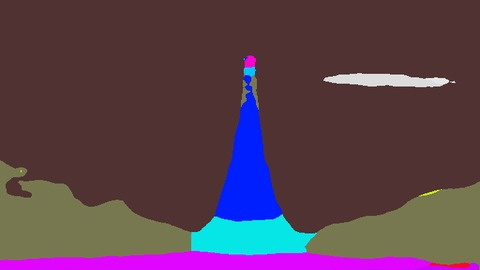
\includegraphics[width=1\linewidth]{reference_seg_paris.jpg}
	\caption{Reference Image Segmentation}
\end{subfigure}
\begin{subfigure}[t]{0.3\linewidth}
	\centering
	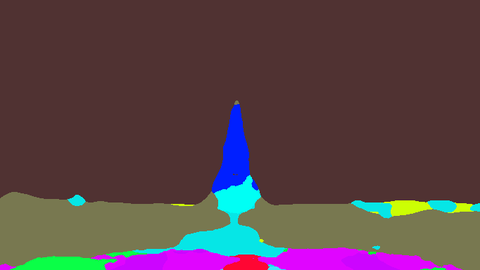
\includegraphics[width=1\linewidth]{out0052.png}
	\caption{Content Frame 52 Segmentation}
\end{subfigure}
\caption{Eiffel Tower photorealistic video style transfer results.}
\end{figure}
The algorithm successfully transfers the general colour of the sky, and the ground lighting. The lighting of the tower is only partially transferred. This was due to the segmentation method failing to classify the top of the tower as a building (dark blue), instead losing it amongst the sky segment as seen in Figure 1i. The output frames successfully track the motion of the sky, as well as vehicles around the base of the tower. While general motion is minimal, we show that our algorithm produces consistent output without temporal artifacts.

Having shown consistent landscape photorealistic style transfer, the algorithm was applied to a scene with a higher degree of movement. Here, a summer video of cars racing down a road has its season transformed later into fall.
\begin{figure}[h!]
\centering
\begin{subfigure}[t]{0.3\linewidth}
    \centering
    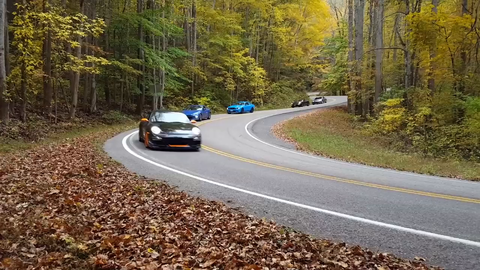
\includegraphics[width=1\linewidth]{cars/small_0035.png}
    \caption{Content Frame 35}
\end{subfigure}
\begin{subfigure}[t]{0.3\linewidth}
    \centering
    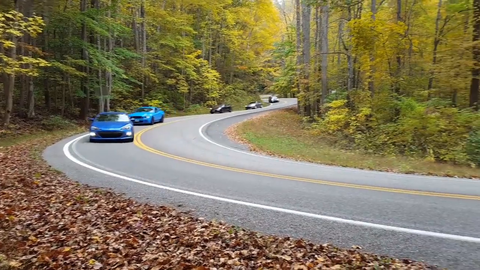
\includegraphics[width=1\linewidth]{cars/small_0054.png}
    \caption{Content Frame 54}
\end{subfigure}
\begin{subfigure}[t]{0.3\linewidth}
    \centering
    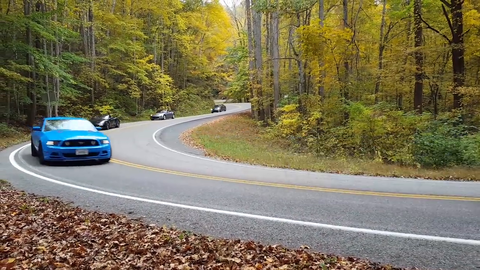
\includegraphics[width=1\linewidth]{cars/small_0082.png}
    \caption{Content Frame 82}
\end{subfigure}

\begin{subfigure}[t]{0.3\linewidth}
    \centering
    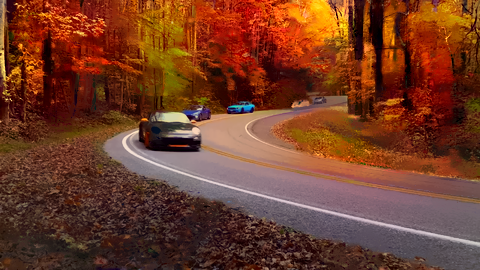
\includegraphics[width=1\linewidth]{cars/best35.png}
    \caption{Output Frame 35}
\end{subfigure}
\begin{subfigure}[t]{0.3\linewidth}
    \centering
    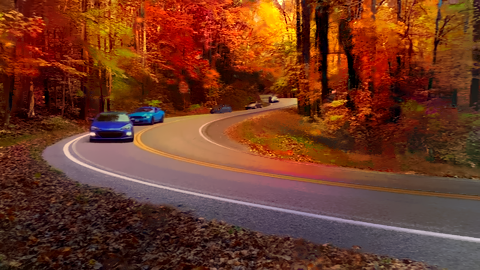
\includegraphics[width=1\linewidth]{cars/best54.png}
    \caption{Output Frame 54}
\end{subfigure}
\begin{subfigure}[t]{0.3\linewidth}
    \centering
    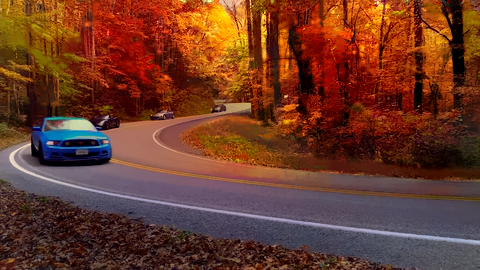
\includegraphics[width=1\linewidth]{cars/best82.png}
    \caption{Output Frame 82}
\end{subfigure}
\begin{subfigure}[t]{0.3\linewidth}
    \centering
    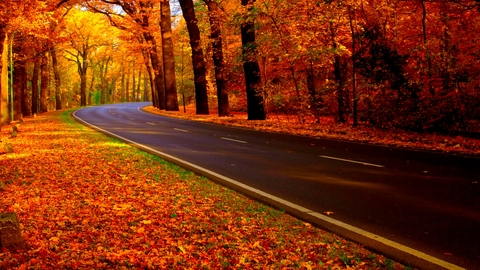
\includegraphics[width=1\linewidth]{cars/reference.jpg}
    \caption{Reference Image}
\end{subfigure}
\begin{subfigure}[t]{0.3\linewidth}
	\centering
	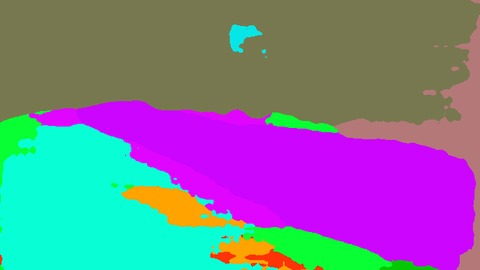
\includegraphics[width=1\linewidth]{reference_seg_cars.jpg}
	\caption{Reference Image Segmentation}
\end{subfigure}
\begin{subfigure}[t]{0.3\linewidth}
	\centering
	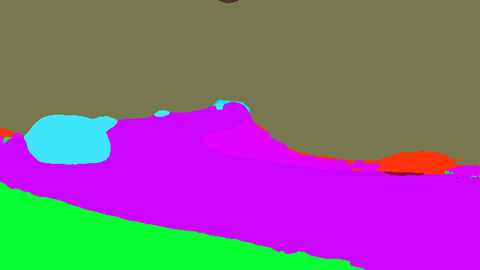
\includegraphics[width=1\linewidth]{cars/out0082.png}
	\caption{Content Frame 82 Segmentation}
\end{subfigure}
\caption{Cars in a forest photorealistic video style transfer results.}
\vspace{-0.2cm}
\end{figure}
The leaf colour of the trees was successfully transferred from the reference image. Also the tree trunk colour was changed as the tree species are different between the reference image and the content video. More importantly, the cars were left unaffected as no reference cars were contained in the reference image. For this example the reference segmentation was manually touched up to improve results. This requires minimal time to do as there is only one reference frame.


\section{Conclusion}
\vspace{-0.2cm}
Two previous style transfer works were introduced. We then produced a novel combination of these two paper's loss functions to bring photorealistic style transfer to video content. This is our most significant contribution. We know of no previous work that achieves this same task. By successfully demonstrating our algorithm we also further validate the results of Ruder et. al. [1] and Luan et al. [4]. Ruder's video style transfer algorithm is shown to be robust enough to be used within other types of style transfer algorithms. Luan's photorealistic style transfer method also produces consistent enough results to successfully stylize multiple frames of video. Issues seen in our results are typically due to poor segmentation. This is a critical area of improvement for future work.

%\subsection{Paper length}
%Papers submitted for review should be complete. 
%The length should match that intended for final publication. 
%Papers accepted for the conference will be allocated 14 pages (plus references) in the proceedings. 
%Note that the allocated 14 pages do not include the references. The reason for this policy
%is that we do not want authors to omit references for sake of space limitations.
%
%Papers with more than 14 pages (excluding references) will be rejected without review.
%This includes papers where the margins and
%formatting are deemed to have been significantly altered from those
%laid down by this style guide.  The reason such papers will not be
%reviewed is that there is no provision for supervised revisions of
%manuscripts. The reviewing process cannot determine the suitability of
%the paper for presentation in 14 pages if it is reviewed in 16.
%
%\subsection{Paper ID}
%
%It is imperative that the paper ID is mentioned on each page of the manuscript.
%The paper ID is a number automatically assigned to your submission when 
%registering your paper submission on CMT.
%
%
%\subsection{Line numbering}
%
%All lines should be numbered, as in this example document.  This makes
%reviewing more efficient, because reviewers can refer to a line on a
%page.  If you are preparing a document using a non-\LaTeX\
%document preparation system, please arrange for an equivalent line numbering.
%
%
%
%\subsection{Mathematics}
%
%Please number all of your sections and displayed equations.  Again,
%this makes reviewing more efficient, because reviewers can refer to a
%line on a page.  Also, it is important for readers to be able to refer
%to any particular equation.  Just because you didn't refer to it in
%the text doesn't mean some future reader might not need to refer to
%it.  It is cumbersome to have to use circumlocutions like ``the
%equation second from the top of page 3 column 1''.  (Note that the
%line numbering will not be present in the final copy, so is not an
%alternative to equation numbers).  Some authors might benefit from
%reading Mermin's description of how to write mathematics:
%\url{www.pamitc.org/documents/mermin.pdf‎}.
%
%\section{Blind review}
%\label{sec:blind}
%
%Many authors misunderstand the concept of anonymizing for blind
%review.  Blind review does not mean that one must remove
%citations to one's own work. In fact it is often impossible to
%review a paper unless the previous citations are known and
%available.
%
%Blind review means that you do not use the words ``my'' or ``our''
%when citing previous work.  That is all.  (But see below for
%technical reports).
%
%Saying ``this builds on the work of Lucy Smith [1]'' does not say
%that you are Lucy Smith, it says that you are building on her
%work.  If you are Smith and Jones, do not say ``as we show in
%[7]'', say ``as Smith and Jones show in [7]'' and at the end of the
%paper, include reference 7 as you would any other cited work.
%
%An example of a bad paper:
%\begin{quote}
%\begin{center}
%    An analysis of the frobnicatable foo filter.
%\end{center}
%
%   In this paper we present a performance analysis of our
%   previous paper [1], and show it to be inferior to all
%   previously known methods.  Why the previous paper was
%   accepted without this analysis is beyond me.
%
%   [1] Removed for blind review
%\end{quote}
%
%
%An example of an excellent paper:
%
%\begin{quote}
%\begin{center}
%     An analysis of the frobnicatable foo filter.
%\end{center}
%
%   In this paper we present a performance analysis of the
%   paper of Smith [1], and show it to be inferior to
%   all previously known methods.  Why the previous paper
%   was accepted without this analysis is beyond me.
%
%   [1] Smith, L. and Jones, C. ``The frobnicatable foo
%   filter, a fundamental contribution to human knowledge''.
%   Nature 381(12), 1-213.
%\end{quote}
%
%If you are making a submission to another conference at the same
%time, which covers similar or overlapping material, you may need
%to refer to that submission in order to explain the differences,
%just as you would if you had previously published related work. In
%such cases, include the anonymized parallel
%submission~\cite{Authors14} as additional material and cite it as
%\begin{quote}
%1. Authors. ``The frobnicatable foo filter'', BMVC 2014 Submission
%ID 324, Supplied as additional material {\tt bmvc14.pdf}.
%\end{quote}
%
%Finally, you may feel you need to tell the reader that more
%details can be found elsewhere, and refer them to a technical
%report.  For conference submissions, the paper must stand on its
%own, and not {\em require} the reviewer to go to a techreport for
%further details.  Thus, you may say in the body of the paper
%``further details may be found in~\cite{Authors14b}''.  Then
%submit the techreport as additional material. Again, you may not
%assume the reviewers will read this material.
%
%Sometimes your paper is about a problem which you tested using a tool which
%is widely known to be restricted to a single institution.  For example,
%let's say it's 1969, you have solved a key problem on the Apollo lander,
%and you believe that the ECCV audience would like to hear about your
%solution.  The work is a development of your celebrated 1968 paper entitled
%``Zero-g frobnication: How being the only people in the world with access to
%the Apollo lander source code makes us a wow at parties'', by Zeus.
%
%You can handle this paper like any other.  Don't write ``We show how to
%improve our previous work [Anonymous, 1968].  This time we tested the
%algorithm on a lunar lander [name of lander removed for blind review]''.
%That would be silly, and would immediately identify the authors. Instead
%write the following:
%\begin{quotation}
%\noindent
%   We describe a system for zero-g frobnication.  This
%   system is new because it handles the following cases:
%   A, B.  Previous systems [Zeus et al. 1968] didn't
%   handle case B properly.  Ours handles it by including
%   a foo term in the bar integral.
%
%   ...
%
%   The proposed system was integrated with the Apollo
%   lunar lander, and went all the way to the moon, don't
%   you know.  It displayed the following behaviours
%   which show how well we solved cases A and B: ...
%\end{quotation}
%As you can see, the above text follows standard scientific convention,
%reads better than the first version, and does not explicitly name you as
%the authors.  A reviewer might think it likely that the new paper was
%written by Zeus, but cannot make any decision based on that guess.
%He or she would have to be sure that no other authors could have been
%contracted to solve problem B. \\
%
%For sake of anonymity, it's recommended to omit acknowledgements
%in your review copy. They can be added later when you prepare the final copy.
%
%
%
%\section{Manuscript Preparation}
%
%This is an edited version of Springer LNCS instructions adapted
%for ECCV 2018 first paper submission.
%You are strongly encouraged to use \LaTeX2$_\varepsilon$ for the
%preparation of your
%camera-ready manuscript together with the corresponding Springer
%class file \verb+llncs.cls+.
%
%We would like to stress that the class/style files and the template
%should not be manipulated and that the guidelines regarding font sizes
%and format should be adhered to. This is to ensure that the end product
%is as homogeneous as possible.
%
%\subsection{Printing Area}
%The printing area is $122  \; \mbox{mm} \times 193 \;
%\mbox{mm}$.
%The text should be justified to occupy the full line width,
%so that the right margin is not ragged, with words hyphenated as
%appropriate. Please fill pages so that the length of the text
%is no less than 180~mm.
%
%\subsection{Layout, Typeface, Font Sizes, and Numbering}
%Use 10-point type for the name(s) of the author(s) and 9-point type for
%the address(es) and the abstract. For the main text, please use 10-point
%type and single-line spacing.
%We recommend using Computer Modern Roman (CM) fonts, Times, or one
%of the similar typefaces widely used in photo-typesetting.
%(In these typefaces the letters have serifs, i.e., short endstrokes at
%the head and the foot of letters.)
%Italic type may be used to emphasize words in running text. Bold
%type and underlining should be avoided.
%With these sizes, the interline distance should be set so that some 45
%lines occur on a full-text page.
%
%\subsubsection{Headings.}
%
%Headings should be capitalized
%(i.e., nouns, verbs, and all other words
%except articles, prepositions, and conjunctions should be set with an
%initial capital) and should,
%with the exception of the title, be aligned to the left.
%Words joined by a hyphen are subject to a special rule. If the first
%word can stand alone, the second word should be capitalized.
%The font sizes
%are given in Table~\ref{table:headings}.
%\setlength{\tabcolsep}{4pt}
%\begin{table}
%\begin{center}
%\caption{Font sizes of headings. Table captions should always be
%positioned {\it above} the tables. The final sentence of a table
%caption should end without a full stop}
%\label{table:headings}
%\begin{tabular}{lll}
%\hline\noalign{\smallskip}
%Heading level & Example & Font size and style\\
%\noalign{\smallskip}
%\hline
%\noalign{\smallskip}
%Title (centered)  & {\Large \bf Lecture Notes \dots} & 14 point, bold\\
%1st-level heading & {\large \bf 1 Introduction} & 12 point, bold\\
%2nd-level heading & {\bf 2.1 Printing Area} & 10 point, bold\\
%3rd-level heading & {\bf Headings.} Text follows \dots & 10 point, bold
%\\
%4th-level heading & {\it Remark.} Text follows \dots & 10 point,
%italic\\
%\hline
%\end{tabular}
%\end{center}
%\end{table}
%\setlength{\tabcolsep}{1.4pt}
%
%Here are
%some examples of headings: ``Criteria to Disprove Context-Freeness of
%Collage Languages'', ``On Correcting the Intrusion of Tracing
%Non-deterministic Programs by Software'', ``A User-Friendly and
%Extendable Data Distribution System'', ``Multi-flip Networks:
%Parallelizing GenSAT'', ``Self-determinations of Man''.
%
%\subsubsection{Lemmas, Propositions, and Theorems.}
%
%The numbers accorded to lemmas, propositions, and theorems etc. should
%appear in consecutive order, starting with the number 1, and not, for
%example, with the number 11.
%
%\subsection{Figures and Photographs}
%\label{sect:figures}
%
%Please produce your figures electronically and integrate
%them into your text file. For \LaTeX\ users we recommend using package
%\verb+graphicx+ or the style files \verb+psfig+ or \verb+epsf+.
%
%Check that in line drawings, lines are not
%interrupted and have constant width. Grids and details within the
%figures must be clearly readable and may not be written one on top of
%the other. Line drawings should have a resolution of at least 800 dpi
%(preferably 1200 dpi).
%For digital halftones 300 dpi is usually sufficient.
%The lettering in figures should have a height of 2~mm (10-point type).
%Figures should be scaled up or down accordingly.
%Please do not use any absolute coordinates in figures.
%
%Figures should be numbered and should have a caption which should
%always be positioned {\it under} the figures, in contrast to the caption
%belonging to a table, which should always appear {\it above} the table.
%Please center the captions between the margins and set them in
%9-point type
%(Fig.~\ref{fig:example} shows an example).
%The distance between text and figure should be about 8~mm, the
%distance between figure and caption about 5~mm.
%\begin{figure}
%\centering
%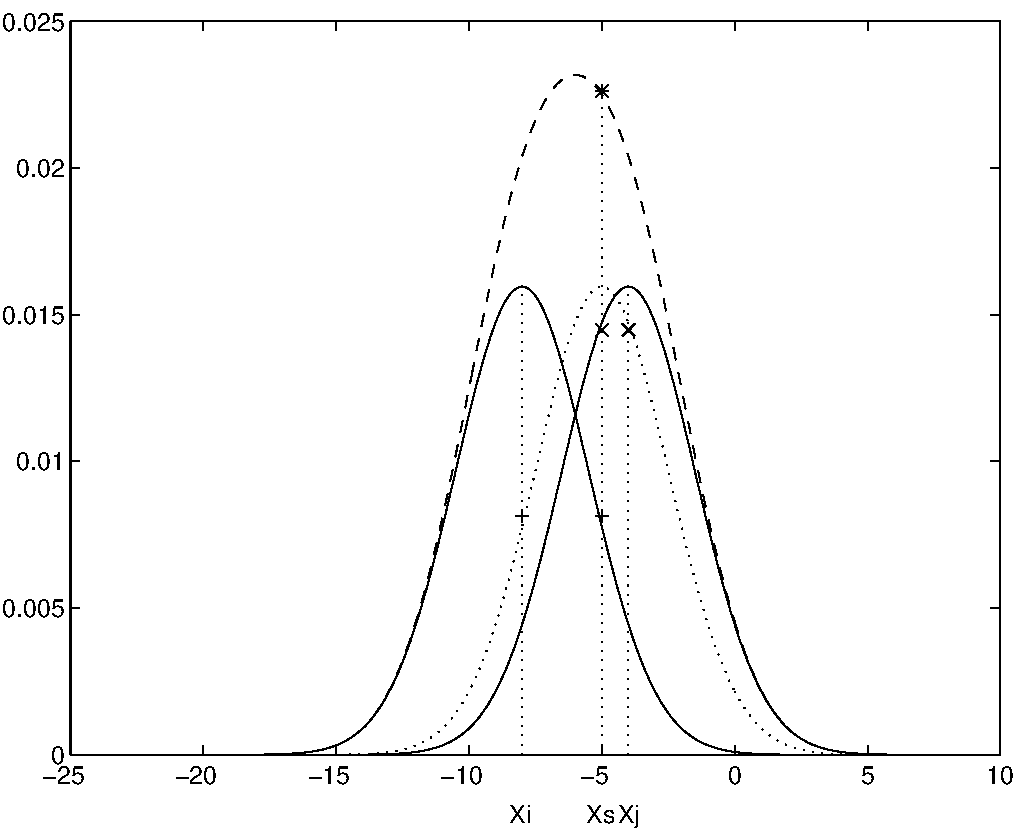
\includegraphics[height=6.5cm]{eijkel2}
%\caption{One kernel at $x_s$ ({\it dotted kernel}) or two kernels at
%$x_i$ and $x_j$ ({\it left and right}) lead to the same summed estimate
%at $x_s$. This shows a figure consisting of different types of
%lines. Elements of the figure described in the caption should be set in
%italics,
%in parentheses, as shown in this sample caption. The last
%sentence of a figure caption should generally end without a full stop}
%\label{fig:example}
%\end{figure}
%
%If possible (e.g. if you use \LaTeX) please define figures as floating
%objects. \LaTeX\ users, please avoid using the location
%parameter ``h'' for ``here''. If you have to insert a pagebreak before a
%figure, please ensure that the previous page is completely filled.
%
%
%\subsection{Formulas}
%
%Displayed equations or formulas are centered and set on a separate
%line (with an extra line or halfline space above and below). Displayed
%expressions should be numbered for reference. The numbers should be
%consecutive within the contribution,
%with numbers enclosed in parentheses and set on the right margin.
%For example,
%\begin{align}
%  \psi (u) & = \int_{0}^{T} \left[\frac{1}{2}
%  \left(\Lambda_{0}^{-1} u,u\right) + N^{\ast} (-u)\right] dt \; \\
%& = 0 ?
%\end{align}
%
%Please punctuate a displayed equation in the same way as ordinary
%text but with a small space before the end punctuation.
%
%\subsection{Footnotes}
%
%The superscript numeral used to refer to a footnote appears in the text
%either directly after the word to be discussed or, in relation to a
%phrase or a sentence, following the punctuation sign (comma,
%semicolon, or full stop). Footnotes should appear at the bottom of
%the
%normal text area, with a line of about 2~cm in \TeX\ and about 5~cm in
%Word set
%immediately above them.\footnote{The footnote numeral is set flush left
%and the text follows with the usual word spacing. Second and subsequent
%lines are indented. Footnotes should end with a full stop.}
%
%
%\subsection{Program Code}
%
%Program listings or program commands in the text are normally set in
%typewriter font, e.g., CMTT10 or Courier.
%
%\noindent
%{\it Example of a Computer Program}
%\begin{verbatim}
%program Inflation (Output)
%  {Assuming annual inflation rates of 7%, 8%, and 10%,...
%   years};
%   const
%     MaxYears = 10;
%   var
%     Year: 0..MaxYears;
%     Factor1, Factor2, Factor3: Real;
%   begin
%     Year := 0;
%     Factor1 := 1.0; Factor2 := 1.0; Factor3 := 1.0;
%     WriteLn('Year  7% 8% 10%'); WriteLn;
%     repeat
%       Year := Year + 1;
%       Factor1 := Factor1 * 1.07;
%       Factor2 := Factor2 * 1.08;
%       Factor3 := Factor3 * 1.10;
%       WriteLn(Year:5,Factor1:7:3,Factor2:7:3,Factor3:7:3)
%     until Year = MaxYears
%end.
%\end{verbatim}
%%
%\noindent
%{\small (Example from Jensen K., Wirth N. (1991) Pascal user manual and
%report. Springer, New York)}
%
%
%
%\subsection{Citations}
%
%The list of references is headed ``References" and is not assigned a
%number
%in the decimal system of headings. The list should be set in small print
%and placed at the end of your contribution, in front of the appendix,
%if one exists.
%Please do not insert a pagebreak before the list of references if the
%page is not completely filled.
%An example is given at the
%end of this information sheet. For citations in the text please use
%square brackets and consecutive numbers: \cite{Alpher02},
%\cite{Alpher03}, \cite{Alpher04} \dots
%
%\section{Conclusions}
%
%The paper ends with a conclusion. 
%
%
%\clearpage\mbox{}Page \thepage\ of the manuscript.
%\clearpage\mbox{}Page \thepage\ of the manuscript.
%\clearpage\mbox{}Page \thepage\ of the manuscript.
%\clearpage\mbox{}Page \thepage\ of the manuscript.
%\clearpage\mbox{}Page \thepage\ of the manuscript.
%\clearpage\mbox{}Page \thepage\ of the manuscript.
%\clearpage\mbox{}Page \thepage\ of the manuscript.
%This is the last page of the manuscript.
%\par\vfill\par
%Now we have reached the maximum size of the ECCV 2018 submission (excluding references).
%References should start immediately after the main text, but can continue on p.15 if needed.
%
%\clearpage
%
\bibliographystyle{splncs}
\bibliography{egbib}
\end{document}
